\section{実験手法}
\subsection{電流パルスを用いたα相からβ相への変換}
まず、試料に電流パルスを印加してオーム発熱により加熱し、α相からβ相に相転移を起こすことを目標とした。相転移の確認は、パルス印加中の抵抗変化を測定することで行った。その際用いた電気回路の模式図を図\ref{fig:schematics_pulse}に示す。ソースメータ(Keithley 2400)から出力されたパルス電圧は、パワーアンプ(NF Corp. 4502)で100倍に増幅されたあと、光学クライオスタット中の試料とロード抵抗の直列接続に印加される。回路に流れる電流の時間変化は、$\rm 5.4\Omega$のロード抵抗の電圧降下をデータロガー(MC DT8824)で読み取り計算した(Ch2)。また試料の電圧降下もデータロガー(MC DT8824)で読み取り計算した(Ch1)
\begin{figure}[!h]
    \begin{center}
   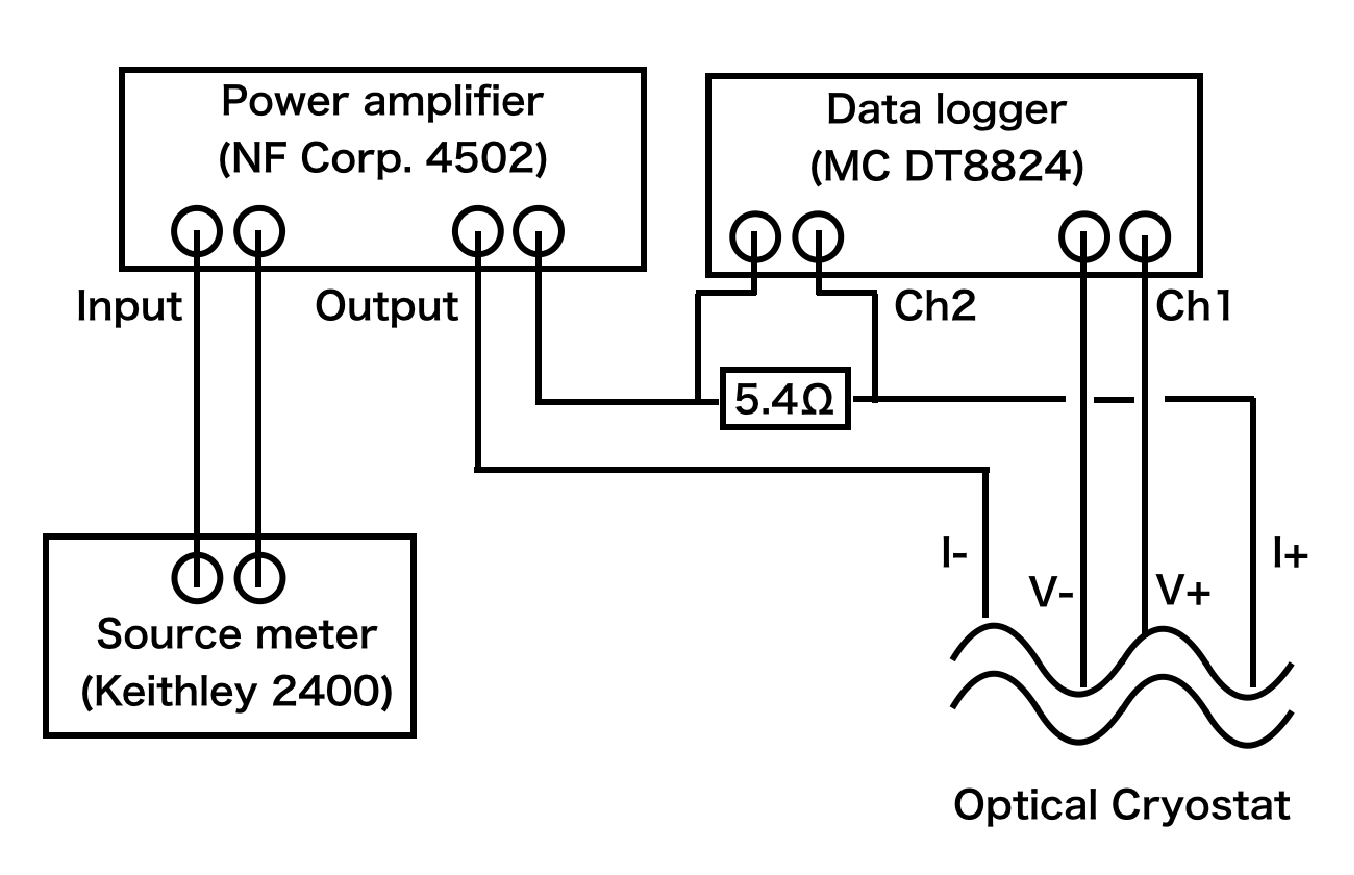
\includegraphics[width=0.5\hsize]{experiment/schematics_pulse.eps}
  \end{center}
  \caption{}
  \label{fig:schematics_pulse}
  \end{figure}
  
相転移には大きな体積変化が伴うため、電流パルスにより試料の温度を上げて相転移を起こし、端子がくっついた状態を維持するためにはいくつかの技術的な工夫が欠かせない。まず筆者は直径$\rm 25 \mu m$の金線を電圧・電流端子として銀ペーストで試料に接続した。その試料を25Kに保持し電流パルスを印加したところ、試料が相転移温度に達するまえに直径$\rm 25 \mu m$の金線からなる電流端子が焼き切れた。そのときの電流は1.3A程度だった。したがって電流端子に繋ぐ金線は$\rm 25 \mu m$より太いものに取り替える必要がある。また数A程度の電流を流すと試料付近以外で発熱し断線のリスクがあるため、あえて高抵抗(ヒーター)の領域を作って試料付近の発熱効率を高める必要がある。そこで、次に筆者はカーボンペーストで直径$\rm 50 \mu m$の金線を接続することで、効果的に試料を加熱しながら、かつ金線が焼き切れないような構成を目指した。しかしこの構成では試料が相転移温度に達するまえに、カーボンペーストによる接続部が過熱で壊れてしまった。この結果はカーボンペーストは銀ペーストに比べ抵抗が高い反面、機械強度が弱いことに起因する。またカーボンペーストを用いた電気的な接続ではカーボンペーストの高い抵抗率に起因して、発熱部分が試料と金線の間に集中してしまう。

筆者は以上に述べたような試行錯誤の結果、図\ref{fig:schematics_sample}のような端子の接続法を見出した。前述したように、カーボンペーストは発熱に十分に高い抵抗が実現できる一方で機械的な強度が低く、銀ペーストは強度が高い一方で抵抗が小さい。これらを効果的に組み合わせることで、筆者は機械的強度と高抵抗を確保できると筆者は考えた。そこでカーボンペーストで金線をコーティングした後、銀ペーストで覆い試料にしっかりと接続した。この構成では低抵抗率の銀ペーストが挟まっているので試料と金線の間に電流経路が集中せず、比較的一様な発熱が可能となったと考える。また電流端子につなぐ金線は1A程度以下の電流で焼き切れないように直径$\rm 50 \mu m$のものとした。一方、電圧端子をつなぐ線には大電流が流れないため、柔らかく熱伝導の高すぎないものとしたかった。そこで直径$\rm 25 \mu m$の金線とした。
\begin{figure}[!h]
    \begin{center}
   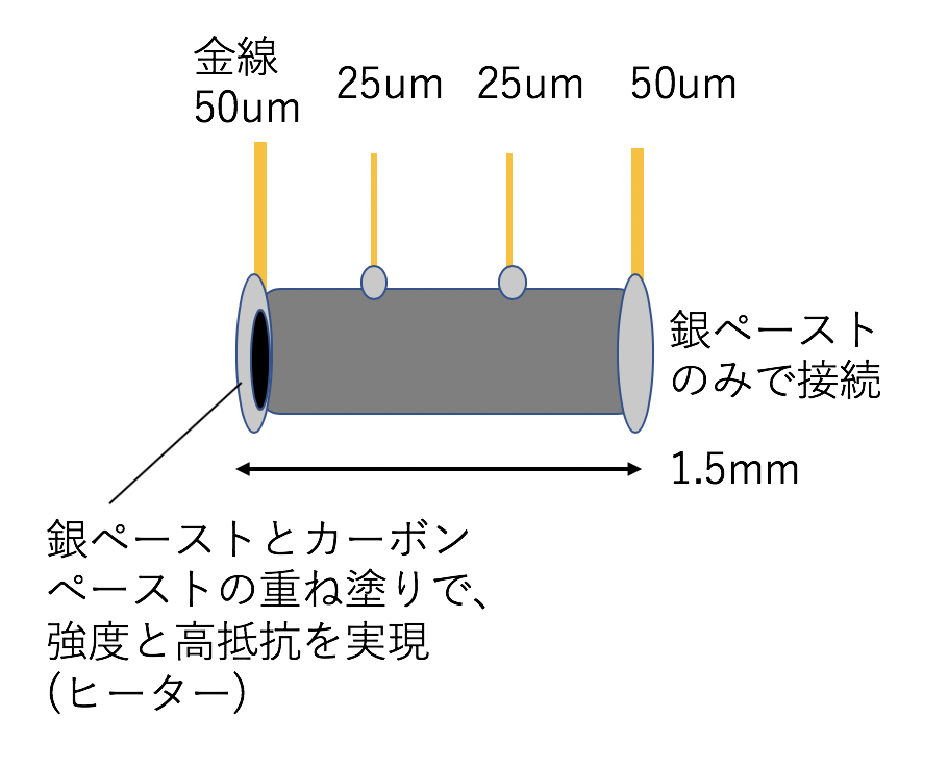
\includegraphics[width=0.4\hsize]{experiment/schematics_sample.eps}
  \end{center}
  \caption{}
  \label{fig:schematics_sample}
\end{figure}

またパルス印加の前後に抵抗の温度依存性も測定した。抵抗の温度依存性を測定するときの電気回路の模式図を図\ref{fig:schematics_lockin}に示す。ロックインアンプ(Stanford Research SR830)から出力した105Hzの交流電圧は、光学クライオスタット中の試料とロード抵抗の直列接続に印加される。回路に流れる電流は$\rm 150\Omega$のロード抵抗の電圧降下をマルチメータ(Keithley 2001)で読み取り算出した。試料の電圧端子間の電圧効果はトランス増幅器(Stanford Research SR554)で100倍に増幅したあと、ロックインアンプの入力端子に入力した。回路に流す電流値は、25Kの試料にパルス電流を印加したとき温度上昇しなかった値より十分小さくとった。また試料の複素インピーダンスの虚部(位相進み/遅れ)成分は実部の1/100程度以下だったので無視して、実部のみを抵抗とした。
\begin{figure}[!h]
     \begin{center}
   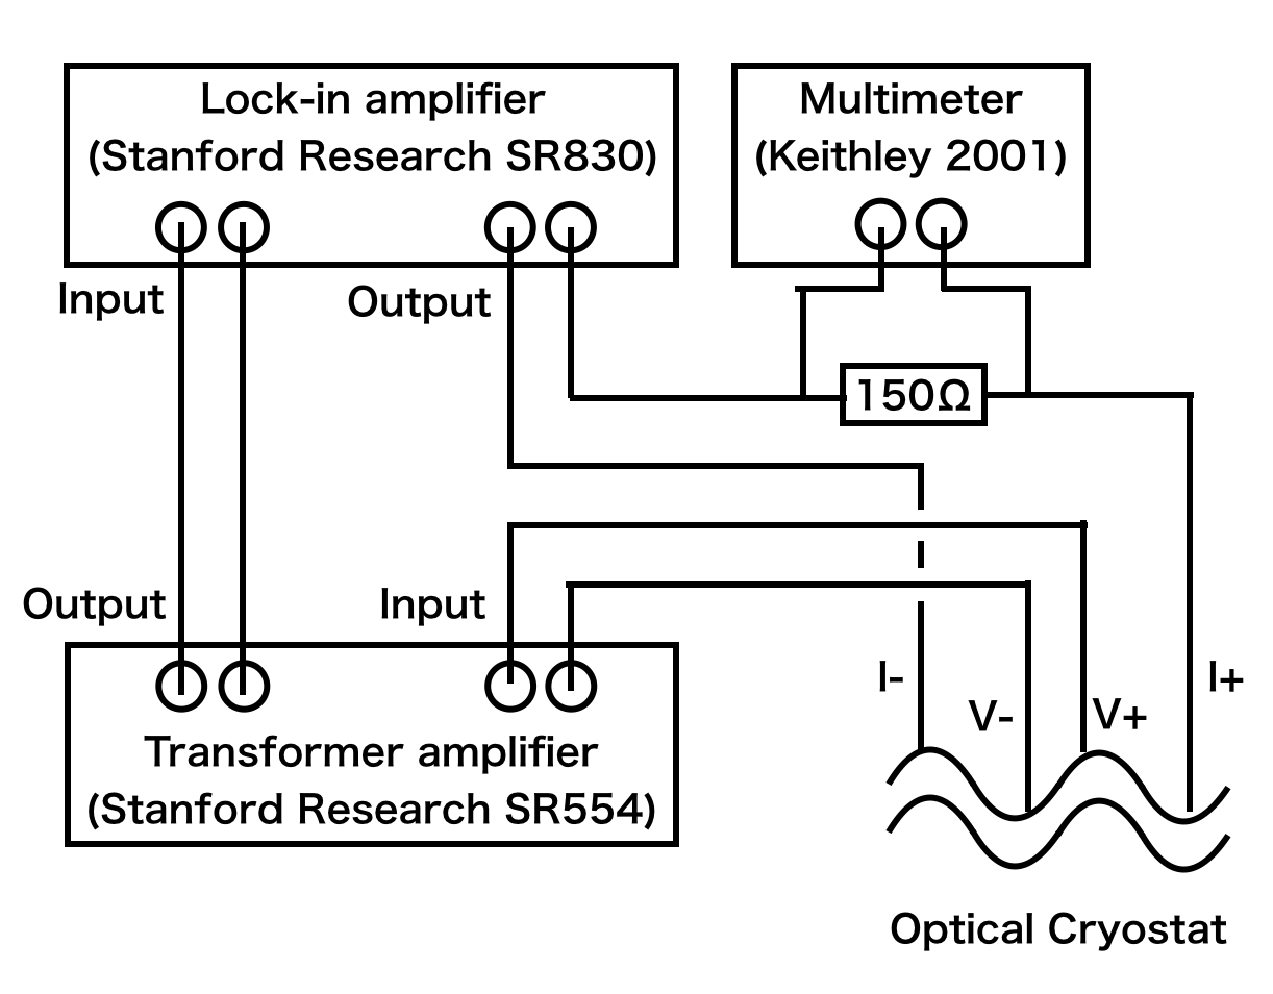
\includegraphics[width=0.5\hsize]{experiment/schematics_lockin.eps}
  \end{center}
  \caption{}
  \label{fig:schematics_lockin}
\end{figure}


\subsection{電流パルスによるαスズとβスズの共存状態の生成}
次に試料に電流パルスを印加してαスズを部分的にβスズに変換し、αスズとβスズの共存状態を生成することを目指した。本実験のセットアップは前節と同様である。ただし顕微光学系を構成しパルス印加中の試料を光学的に観察した点と、図\ref{fig:schematics_sample2}のように電流端子の片側のみにカーボンペーストを用いた点が異なる。カーボンペーストを用いて接続する方法は前節と同様である。主に片側のみから発熱させることで意図的に試料内の温度勾配を作り出し、部分的な書き込みを制御した。
\begin{figure}[!h]
 \begin{minipage}{0.4\hsize}
    \begin{center}
   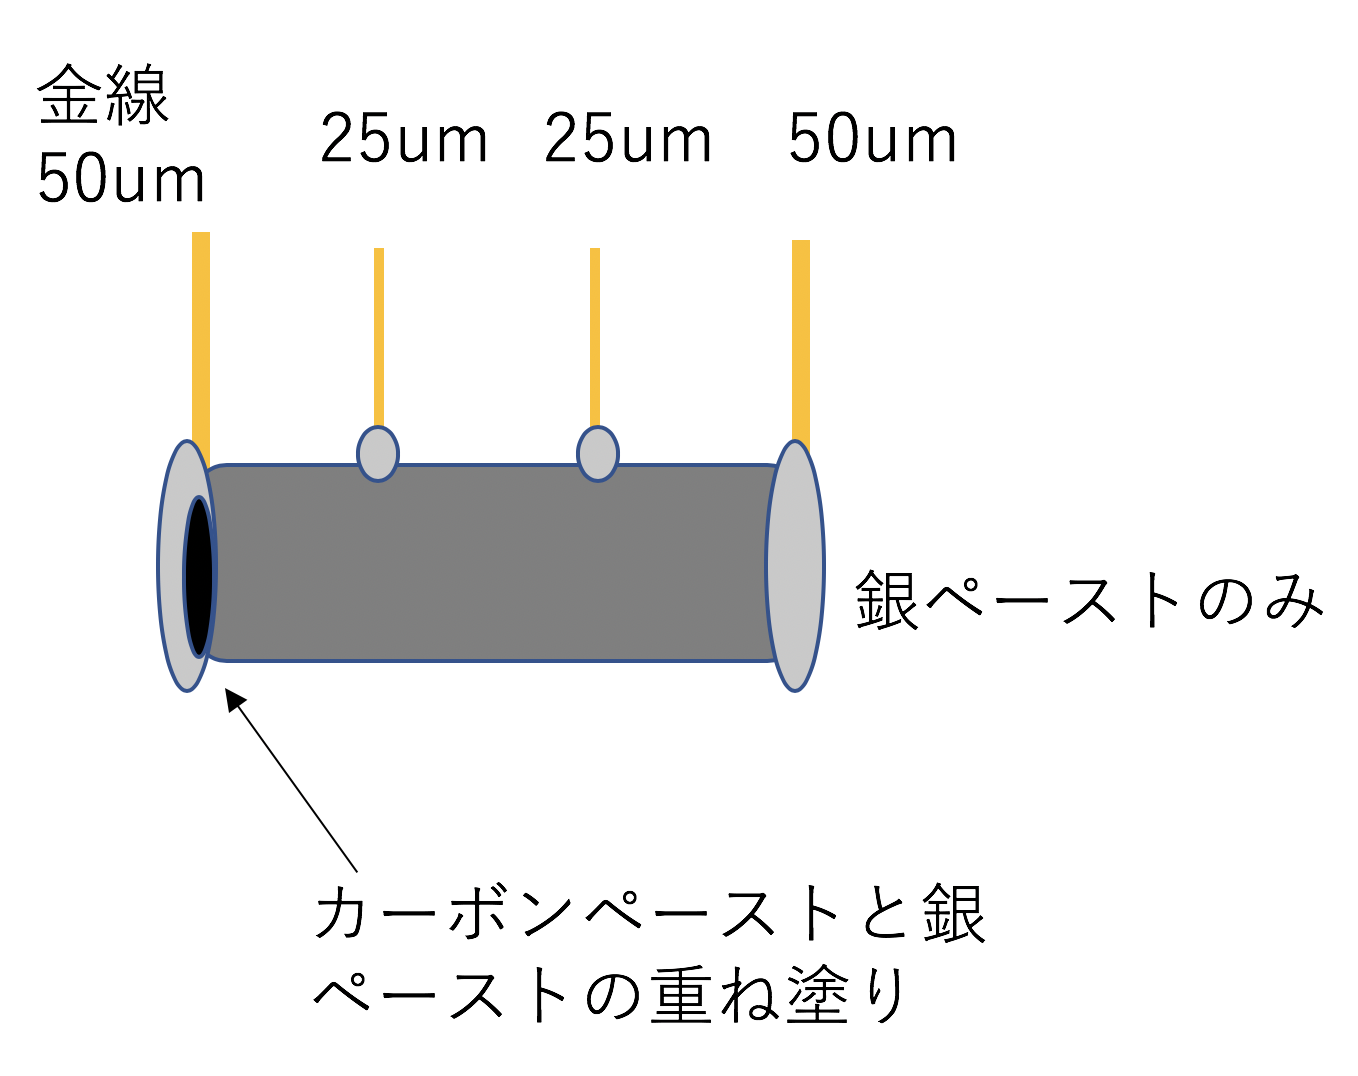
\includegraphics[width=\hsize]{experiment/schematics_sample2.eps}
  \end{center}
  \caption{}
  \label{fig:schematics_sample2}
 \end{minipage}
 \begin{minipage}{0.5\hsize}
     \begin{center}
   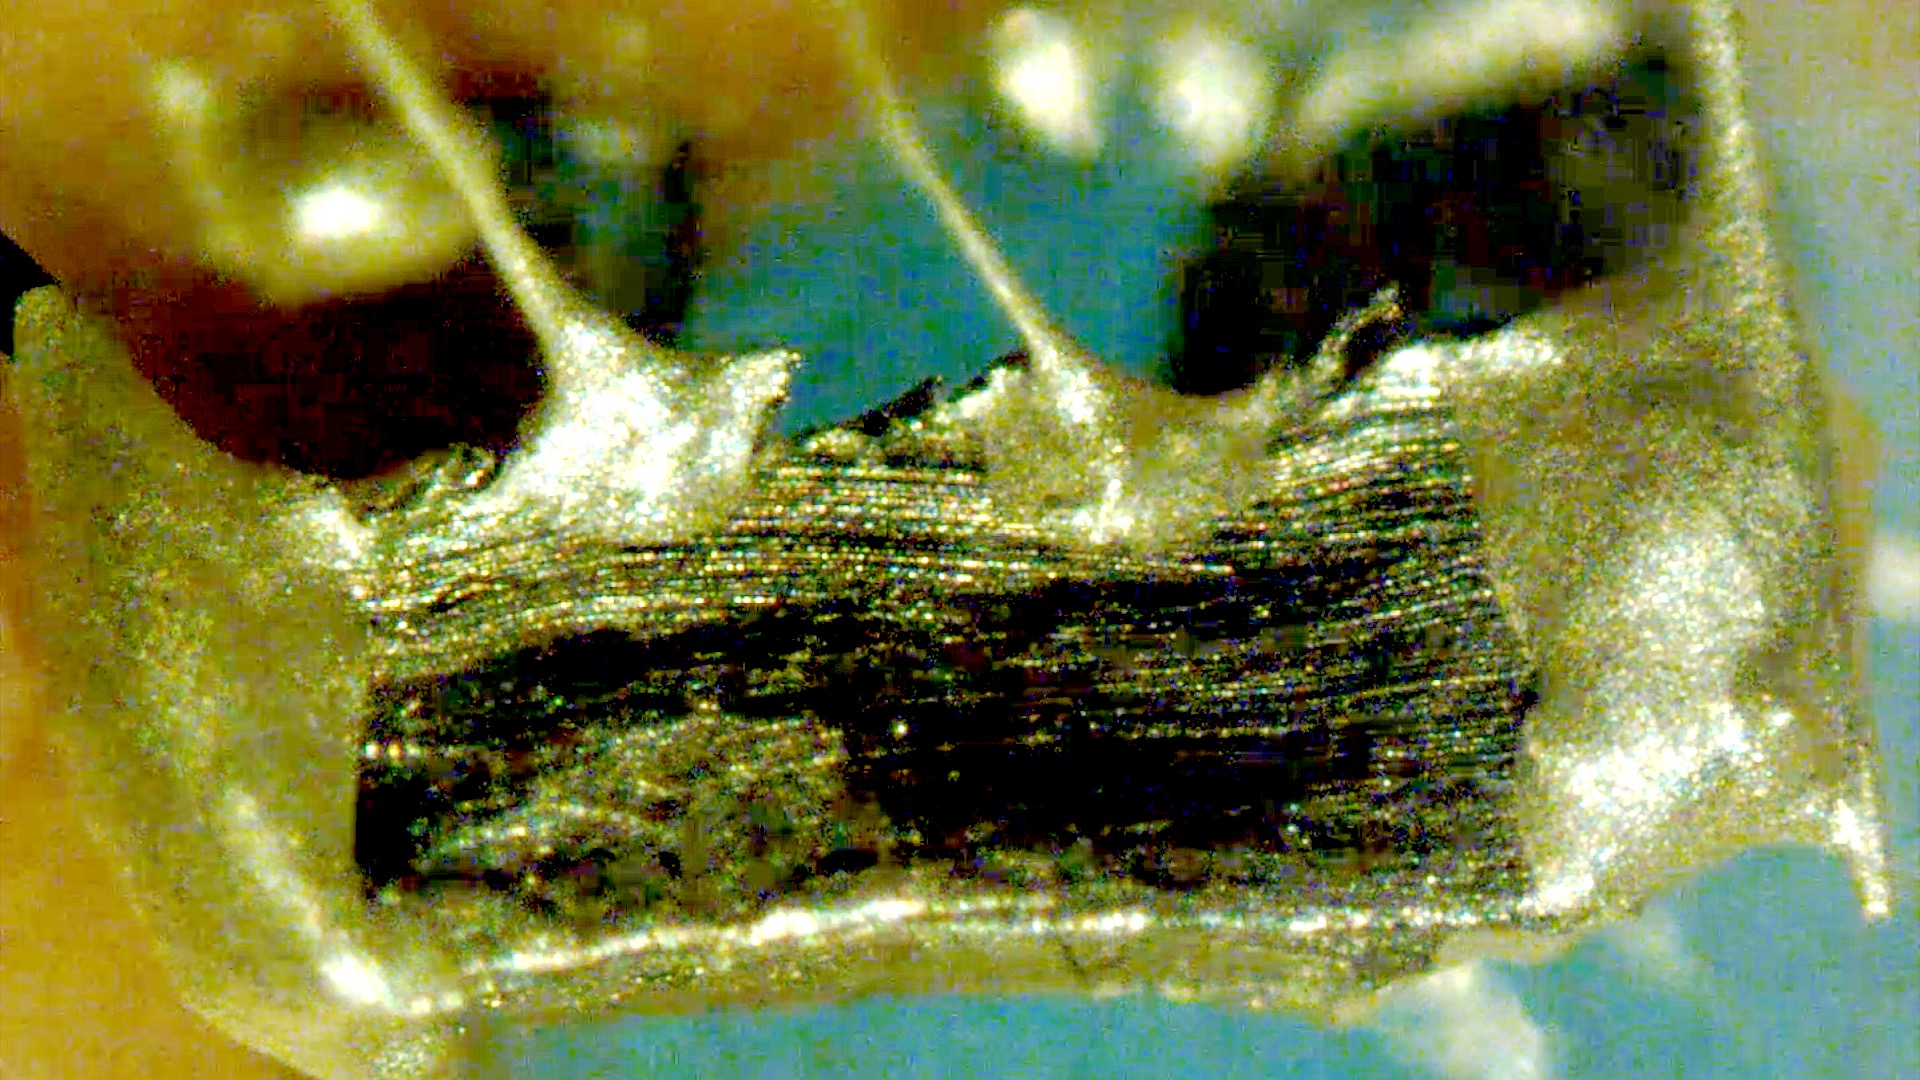
\includegraphics[width=\hsize]{experiment/picture_sample.eps}
  \end{center}
  \caption{ \textcolor{red}{スケールバーが必要}}
  \label{fig:picture_sample}
   \end{minipage}
\end{figure}

%\subsection{電流パルスを用いたβ相からα相への変換}

\clearpage

%\ref{sec:4terminal}